\chapter{Метод нечеткого вывода на основе нечеткого значения истинности}\label{ch:ch2}

\section{Постановка задачи нечеткого вывода}

Лингвистическая модель представляет собой базу правил вида:
\begin{equation}
\label{eqn:fuz-problem-1}
R_k:\ \text{Если}\ x_1\ \text{есть}\ A_{k1}\ \text{и}\ x_2\ \text{есть}\ A_{k2}\ \text{и} \dots \text{и}\ x_n\ \text{есть}\ A_{kn}, \text{то}\ y\ \text{есть}\ B_k,
\end{equation}
где $N$ "--- количество нечетких правил, $A_{ki} \subseteq X_i, i=\overline{1,n}, B_k \subseteq Y$"--- нечеткие множества, которые характеризуются функциями принадлежности $\mu_{A_{ki}}(x_i)$ и $\mu_{B_k}(y)$ соответственно; $x_1, x_2,…,x_n$"--- входные переменные лингвистической модели, причем
\[
[x_1, x_2, ..., x_n]^T = \mathbf{x} \in X_1 \times X_2 \times \dots \times X_n.
\]

Символами  $X_i, i=\overline{1,n}$ и $Y$ обозначаются соответственно пространства входных и выходной переменных. Если ввести обозначения $\mathbf{X}=X_1 \times X_2 \times \dots \times X_n$ и $\mathbf{A_k}=A_{k1}\times A_{k2} \times \dots \times A_{kn}$ , причем
\[
\mu_\mathbf{A_k}(\mathbf{x}) = \underset{i=\overline{1,n}}{T_1} \mu_{A_{ki}}(x_i),
\]
где $T_1$ - произвольная $t$-норма, то правило \ref{eqn:2.1} представляется в виде нечеткой импликации
\begin{equation}
\label{eqn:fuz-problem-2}
R_k: \mathbf{A_k} \to B_k, k=\overline{1,N}.
\end{equation}

Правило $R_k$ можно формализовать как нечеткое отношение, определенное на множестве  $\mathbf{X}\times Y$, т.е. $R_k \subseteq \mathbf{X} \times Y$ - нечеткое множество с функцией принадлежности
\[
\mu_{R_k}(\mathbf{x}, y) = \mu_{\mathbf{A_k} \to B_k} (\mathbf{x}, y).
\]

Модель логического типа определяет задание функции $\mu_{\mathbf{A_k} \to B_k} (\mathbf{x}, y)$ на основе известных функций принадлежности $\mu_{\mathbf{A_k}}(\mathbf{x})$ и $\mu_{B_k}(y)$ с помощью одной из предложенных в [2] функций импликации:
\[
\mu_{\mathbf{A_k} \to B_k} (\mathbf{x}, y) = I(\mu_{\mathbf{A_k}}(\mathbf{x}), \mu_{B_k}(y)),
\]
где $I$"--- некоторая импликация.

Ставится задача определить нечеткий вывод $B'_k \subseteq Y$ для системы, представленной в виде (\ref{eqn:2.1}), если на входах - нечеткие множества.
$\mathbf{A'}=A'_1 \times A'_2 \times \dots \times A'_n \subseteq \mathbf{X}$ или $x_1\ \text{есть}\ A'_1\ \text{и}\ x_2\ \text{есть}\ A'_2\ \text{и} \dots \text{и}\ x_n\ \text{есть}\ A'_n$  с соответствующей функцией принадлежности $\mu_{\mathbf{A'}}(\mathbf{x})$, которая определяется как
\begin{equation}
\label{eqn:fuz-problem-3}
\mu_{\mathbf{A'}}(\mathbf{x}) = \underset{i=\overline{1,n}}{T_3} \mu_{A'_i}(x_i).
\end{equation}

Несинглтонный фаззификатор отображает измеренное $x_i=x'_i, i=\overline{1,n}$ в нечеткое число, для которого $\mu_{A'_i}(x'_i) = 1$ и $\mu_{A'_i}(x_i)$ уменьшается от единицы по мере удаления от  $x'_i$.
В соответствии с обобщенным нечетким правилом modus ponens [2], нечеткое множество $B'_k$ определяется композицией нечеткого множества $\mathbf{A'}$ и отношения $\mathbf{R_k}$, т.е.
\[
B'_k = \mathbf{A'} \circ (\mathbf{A_k} \to B_k),
\]
или, на уровне функций принадлежности
\begin{equation}
\label{eqn:fuz-problem-4}
\mu_{B'_k}(y|\mathbf{x'}) = \sup_{\mathbf{x}\in \mathbf{X}}\left\{\mu_{\mathbf{A'}}(\mathbf{x'})\overset{T_2}{\star} I(\mu_{\mathbf{A_k}}(\mathbf{x}), \mu_{B_k}(y))\right\}.
\end{equation}

В (\ref{eqn:fuz-problem-4}) применена условная нотация, так как ввод в нечеткую систему происходит при определенном значении $\mathbf{x}$, а именно $\mathbf{x'}$. Обозначение $\mu_{B'_k}(y | \mathbf{x'})$ показывает, что $\mu_{B'_k}$ изменяется с каждым значением $\mathbf{x'}$. Вычислительная сложность выражения (\ref{eqn:fuz-problem-4}) составляет $O(|X_1|\cdot |X_2|\cdot \dots \cdot |X_n|\cdot |Y|)$ т.е. экспоненциальная. 

\section{Вывод на основе нечеткого значения истинности}

Используя правило истинностной модификации [1] можно выразить:
\[
\mu_{A'}(\mathbf{x}) = \tau_{A|A'}(\mu_A(x))
\]
где $\tau_{A|A'}$ "--- нечеткое значение истинности (НЗИ) нечеткого множества $A$ относительно $A'$, представляющее собой функцию принадлежности совместимости $CP(A_k, A')$ $A_k$по отношению к $A'$, причем $A'$ рассматривается как достоверное [Дюбуа и др., 1990]:
\begin{equation}
\label{eqn:ftv-compute-12}
\tau_{A_k|A'}(v) = \mu_{CP(A_k, A')}(v) = \sup_{\substack{\mu_{A_k}(x) = v \\ x \in X}} \left\{ \mu_{A'}(x)\right\}.
\end{equation}

Таким образом НЗИ отражает совместимость факта с посылкой в нечеткой форме. Упрощенные подходы отображают совместимость в одно значение из диапазона впервые представленное в [5].

Перейдем от переменной $x$ к переменной $v$ в выражении нечеткого вывода (\ref{}), обозначив
\[
\mu_{A_k}(x) = v \textrm{ и } \mu_{A'}(x) = \tau_{A_k|A'}(v),
\]
то есть выполним преобразование нечетких множеств на пространстве $X$ в истинностное пространство $[0, 1]$:
\[
?????
\]

Получим:
\begin{equation}
\label{eqn:ftv-compute-4}
\mu_{A'}(x) = \tau_{A_k|A'}(\mu_{A_k}(x)) = \tau_{A_k|A'}(v)
\end{equation}

Тогда (\ref{eqn:fuz-problem-4}) примет вид:
\begin{equation}
\label{eqn:ftv-compute-5}
\mu_{B'_k}(y|\mathbf{x'}) = \sup_{v \in [0,1]}\left\{\tau_{A_k|A'}(v) \overset{T_2}{\star} I(v, \mu_{B_k}(y))\right\}.
\end{equation}

При переходе к нечеткому выводу по $n$ входам формула вычисления НЗИ для нечетких отношений посылки и факта имеет вид:
\begin{equation*}
\tau_{\mathbf{A_k}|\mathbf{A'}}(v) = \sup_{\substack{\mu_{\mathbf{A_k}}(x_1, \dots, x_n) = v \\ (x_1, \dots, x_n) \in \mathbf{x}}} \left\{\mu_{\mathbf{A'}}(x_1, \dots, x_n)\right\} .
\end{equation*}

Или в выражении через операции сверток $t$-норм $T_1$ (\ref{eqn:fuz-problem-2}) и $T_3$ (\ref{eqn:fuz-problem-3}):
\begin{equation}
\label{eqn:ftv-compute-6}
\tau_{\mathbf{A_k}|\mathbf{A'}}(v) = \sup_{\substack{\underset{i=\overline{1,n}}{\mathrm{T_1}}\mu_{A_{ki}}(x_i)=v \\ (x_1, \dots, x_n) \in \mathbf{x}}} \left\{ \underset{i=\overline{1,n}}{\mathrm{T_3}} \mu_{A'_i}(x_i) \right\}.
\end{equation}

Вместо выражения (\ref{eqn:ftv-compute-6}), НЗИ для $n$ входов может быть вычислено как свертка НЗИ по каждому отдельному входу:
\begin{equation}
\label{eqn:ftv-compute-7}
\tau_{\mathbf{A_k}|\mathbf{A'}}(v) = \underset{i=\overline{1,n}}{\mathrm{\tilde{T}}} \tau_{A_{ki}|A'_i}, v \in [0, 1],
\end{equation}
где $\mathrm{\tilde{T}}$ - расширенная по принципу обобщения $n$-местная $t$-норма \cite{kutsenko2015methods}, которая определяется как
\begin{equation}
\label{eqn:ftv-compute-8}
\underset{i=\overline{1,n}}{\mathrm{\tilde{T}}} \tau_{A_{ki}|A'_i}(v) = \sup_{\substack{\underset{i=\overline{1,n}}{\mathrm{T_1}}v_i = v \\ (v_1, \dots, v_n) \in [0, 1]^n}} \left\{\underset{i=\overline{1,n}}{\mathrm{T_3}}\tau_{A_{ki}|A'_i}(v_i)\right\}
\end{equation}
в результате перехода
\[
\mu_{A_{ki}}(x_i) = v_i \textrm{ и } \mu_{A'_i}(x_i) = \tau_{A_{ki}|A'_i}(v_i).
\]

Тогда для системы с $n$ входами выражения нечеткого вывода на основе НЗИ (\ref{eqn:ftv-compute-5}) примет вид:
\begin{equation}
\label{eqn:ftv-compute-9}
\mu_{B'_k}(y|\mathbf{x'}) = \sup_{v \in [0, 1]} \left\{\tau_{\mathbf{A_k}|\mathbf{A'}}(v) \overset{\mathrm{T_2}}{\star} I(v, \mu_{B_k}(y))\right\}
\end{equation}

Стоит отметить, что выражение (\ref{eqn:ftv-compute-7}) можно записать следующим образом, подчеркнув возможность попарного рекурсивного нахождения свертки НЗИ:
\begin{align*}
\label{eqn:ftv-compute-10}
\tau_{A_k, A'}(v) & = \underset{i=\overline{1,n}}{\mathrm{\tilde{T}_1}}\tau_{A_{ki}|A'_i}(v_i) \\
& = \left(\dots\left(\left(\mu_{CP(A_{k1}, A'_1)}(v_1)\ \mathrm{\tilde{T}_1}\ \mu_{CP(A_{k2}, A'_2)}(v_2)\right)\ \mathrm{\tilde{T}_1}\ \dots \right) \mathrm{\tilde{T}_1}\ \mu_{CP(A_{kn}, A'_n)}\right).
\end{align*}

Для $n=2$, $\mathrm{\tilde{T}}$ записывается как:
\begin{equation}
\underset{i=\overline{1,2}}{\mathrm{\tilde{T}}} \tau_{A_{ki}|A'_i}(v) = \sup_{\substack{v_1 \mathrm{ T_1 } v_2 = v \\ v_1, v_2 \in [0, 1]}} \left\{ \tau_{A_{k1}|A'_1}(v_1) \mathrm{ T_3 } \tau_{A_{k2}|A'_2}(v_2) \right\}, v \in [0,1].
\label{eqn:ftv-compute-11}
\end{equation}

При вербализации импликации в (\ref{eqn:ftv-compute-8}) она представится в виде:
\begin{equation}
\text{Если } \textit{нзи} \text{ есть } \text{ИСТИННО}, \text{ то }\ y\ \text{есть}\ B'_k
\label{eqn:ftv-compute-13}
\end{equation}

Таким образом, (\ref{eqn:ftv-compute-13}) представляет собой еще одну структуру правил в отличие от канонических структур Заде [10] и Такаги-Сугено [9]. Применение данного правила не зависит от количества входов в нечетких системах.

В формуле (\ref{eqn:ftv-compute-9}) данный подход позволяет переместить процесс вывода в единое пространство НЗИ, где функции истинности, в отличии от различных пространств в подходе Заде, могут быть объединены в более эффективный вычислительный процесс.

\begin{figure}
\centering
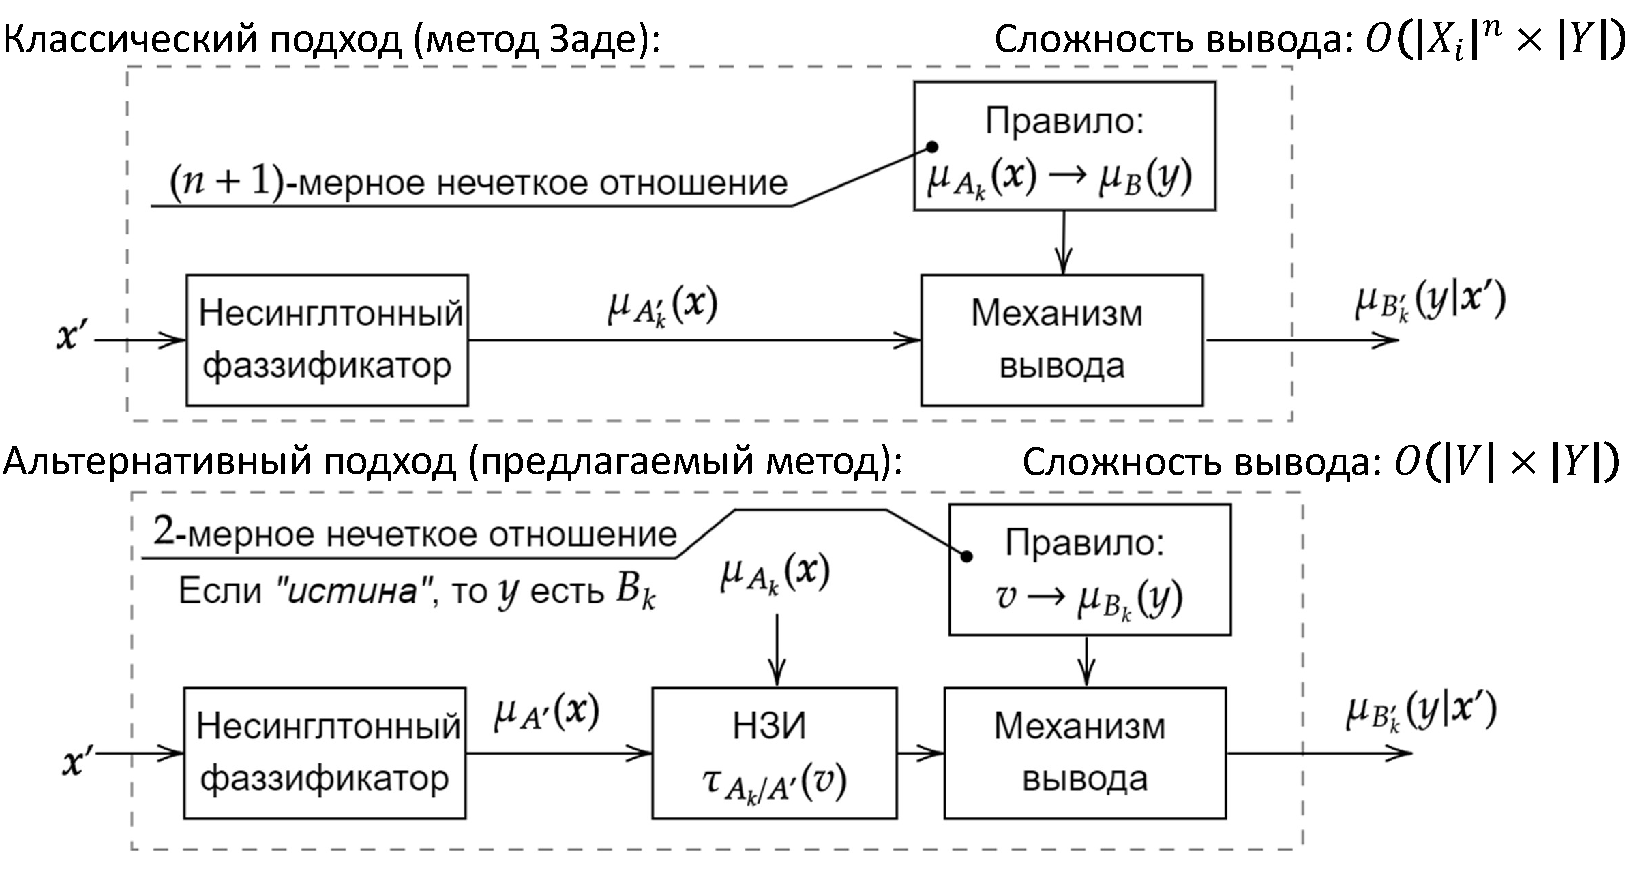
\includegraphics[scale=0.66]{ftv-schema-comparizon}
\caption{Сравнение классической схемы нечеткого вывода и схемы нечеткого вывода на основе НЗИ}
\label{fig:ftv-schema-comparizon}
\end{figure}

Порядок функции временной сложности вычисления $B'_k$ на основе выражения (\ref{eqn:ftv-compute-9}) составляет $O\left(n|V|^2+|V|\cdot |Y|\right)$, где $V=CP(A_k, A')$. Сравнение схем нечетких выводов с соответствии с соотношениями (\ref{eqn:fuz-problem-4}) и (\ref{eqn:ftv-compute-9}) представлены на рис. \cref{fig:ftv-schema-comparizon}.

\section{Вывод для систем логического типа}


\begin{itemize}
	\item S-импликация (Клине-Динеса, Лукасевича, Райхенбаха, Фодора): $I(a, b) = S(1-a, b)$
	\item R-импликация (Гогуен, Гедель): $I(a, b) = \sup_z \left\{z | T(a, z) \le b\right\}$
	\item Q-импликация (Заде, Вильмотта): $I(a, b) = S(1-a, T(a, b))$
\end{itemize}

В логическом подходе правила объединяются связкой <<И>>, тогда результирующее нечеткое множество является результатом произведения нечетких множеств, получаемых в результате нечеткого логического вывода по каждому правилу отдельно:

\begin{eqnarray}
B' = \CapOp_{r=1}^N B'_r.
\end{eqnarray}

\begin{equation}
\mu_{B'}(y) = \Tnorm_{r=1}^N \mu_{B'_r}(y) = \Tnorm_{r=1}^N \left\{\sup_{v\in [0, 1]} \left\{\tau_{A_r|A'}\overset{\mathrm{T}_2}{\star} I\left(v, \mu_{B_r}(y)\right)\right\}\right\}
\end{equation}

%Поскольку импликация в формуле (2.4)  не зависит от входных данных (\ref{eqn:2.2}), то предварительно, т.е. до использования композиционного правила (\ref{eqn:2.5}), вычисляется τ_(k,r) (v)=I(v,μ_(B_k ) (y ̅_r )) при k=(1,N) ̅,r=(1,N) ̅, v∈[0,1].



\section{Анализ эффективности методов нечеткого вывода}

\section{Сравнительный анализ логического подхода к нечетком выводу с подходом Мамдани}

Для формирования условий  в которых тот или иной подход к нечеткому выводу показывает  свои сильные стороны имеет смысл провести сравнение.

\section{Сравнение нечеткого вывода с использованием различных методов дефаззификации}

В статье \cite{VanLeekwijck1999} описывается подход к сравнению методов дефаззификации.

Описанный метод реализации \cite{eisele1994}.

\subsection{Дефаззификация по методу среднего центра}

(center average)

\begin{equation*}
	\label{eqn:defuz-ca-1}
	\hat{y}_{CA} = \frac{\sum_{k=1}^{N} \bar{y}_k \mu_{B'_k}(\bar{y}_k)}{\sum_{k=1}^{N} \mu_{B'_k}(\bar{y}_k)}
\end{equation*}

\begin{figure}[ht]
	\centering
	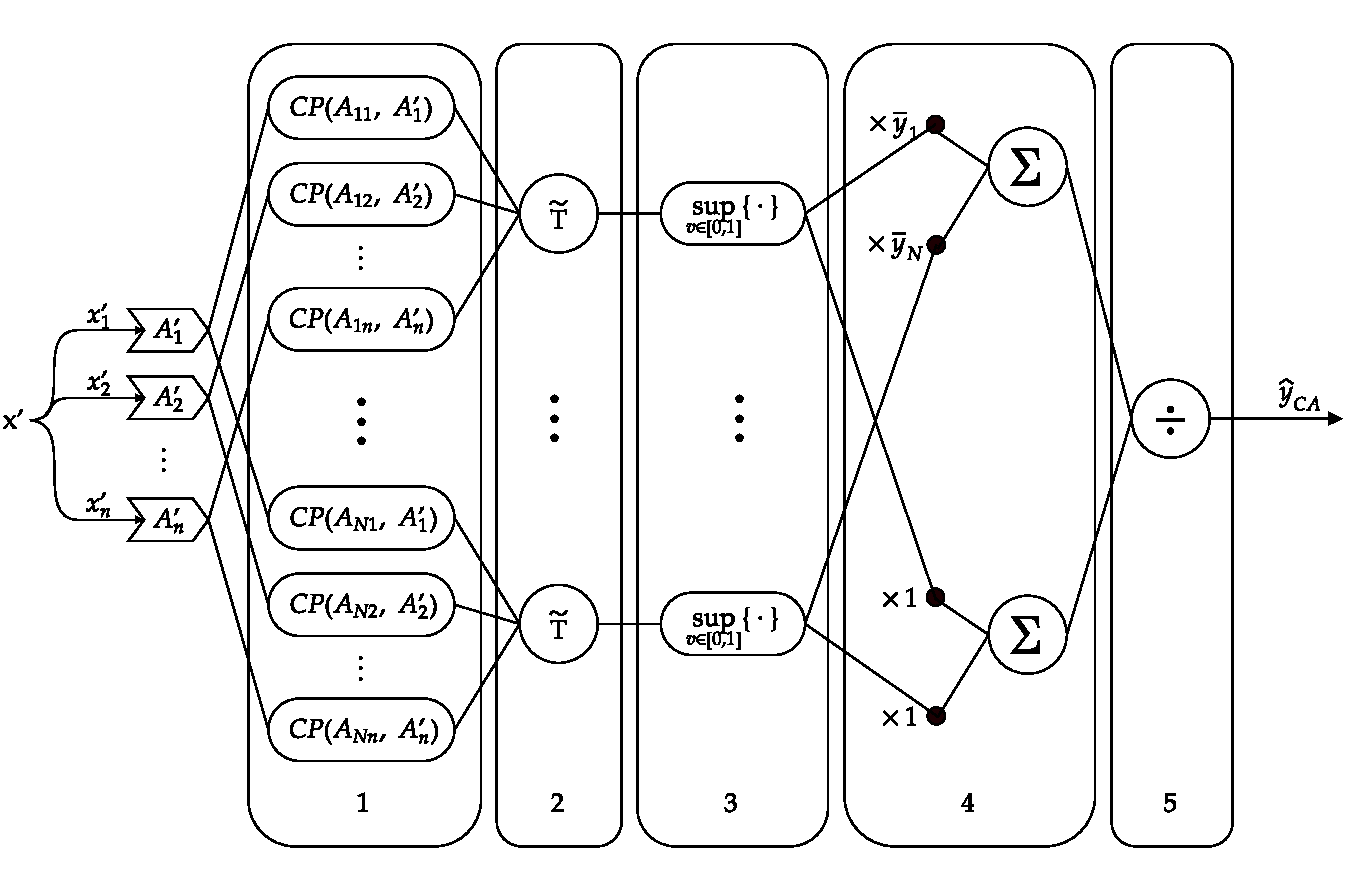
\includegraphics[scale=0.8]{neurofuzzysystem-defuzzification-ca-for-sr-impl}
	\caption{Схема нейро-нечеткой системы с использованием дефаззификации по методу среднего центра для $S$- и $R$-импликаций}
	\label{fig:neurofuzzysystem-defuzzification-ca-for-sr-impl}
\end{figure}

Поскольку $\mu_{B_r}(\overline{y}_k) = 1$ при $k = r$, тогда по формуле (\ref{eqn:ftv-compute-9}) $\mu_{B'_k}(\overline{y}_k)$ выразится:
\begin{align}
	\label{eqn:defuz-ca-3}
	\mu_{B'_k}(\overline{y}_k) &= \sup_{v\in [0, 1]} \left\{\tau_{A_k|A'}\overset{\mathrm{T}_2}{\star} I\left(v, \mu_{B_k}(\overline{y}_k)\right)\right\}\\ &= \sup_{v\in [0, 1]} \left\{\tau_{A_k|A'}\overset{\mathrm{T}_2}{\star} I\left(v, 1\right)\right\}.
\end{align}

Обозначив $I(v, 1) = I_1(v)$, с учетом () формула дефаззификации (\ref{eqn:defuz-ca-3}) примет вид:
\begin{equation}
	\label{eqn:defuz-ca-4}
	\hat{y}_{CA} = \frac{\sum_{k=1}^{N} \bar{y}_k \sup_{v\in [0, 1]} \left\{\tau_{A_r|A'}\overset{\mathrm{T}_2}{\star} I_1(v) \right\}}{\sum_{k=1}^{N} \sup_{v\in [0, 1]} \left\{\tau_{A_r|A'}\overset{\mathrm{T}_2}{\star} I_1(v) \right\}}
\end{equation}

Рассмотрим вычисление $\tau_k$ для различных категорий импликаций:
\begin{itemize}
	\item для \textit{S}-импликаций:
	\begin{align*}
		I_1(v) = I(v, 1) &= S\left\{1-a, 1\right\} = 1\\
	\end{align*}
	\item для \textit{R}-импликаций:
	\begin{align*}
		I_1(v) = I(v, 1) &= \sup_z \left\{z | T(v, z) \le 1\right\}&\quad v\in [0, 1]\\
		&= \sup_z \left\{z | \forall z\right\}&\quad z\in [0, 1]\\
		&= 1
	\end{align*}
	\item для \textit{Q}-импликаций:
	\begin{align*}
		I_1(v) = I(v, 1) &= S\left\{1-v, T(v, 1)\right\}\\
		&= S\left\{1-v, v\right\}\\
	\end{align*}
\end{itemize}


Тогда для \textit{S}- и \textit{R}-импликаций формула (\ref{eqn:defuz-ca-4}) с учетом свойства $t$-нормы $T(a, 1) = a$ примет вид:
\begin{align}
\hat{y}_{CA} &= \frac{\sum_{k=1}^{N} \bar{y}_k \sup_{v\in [0, 1]} \left\{\tau_{\mathbf{A_r}|\mathbf{A'}}\overset{\mathrm{T}_2}{\star} 1 \right\}}{\sum_{k=1}^{N} \sup_{v\in [0, 1]} \left\{\tau_{\mathbf{A_r}|\mathbf{A'}}\overset{\mathrm{T}_2}{\star} 1 \right\}}\\ &= \frac{\sum_{k=1}^{N} \bar{y}_k \sup_{v\in [0, 1]} \left\{\tau_{\mathbf{A_r}|\mathbf{A'}}\right\}}{\sum_{k=1}^{N} \sup_{v\in [0, 1]} \left\{\tau_{\mathbf{A_r}|\mathbf{A'}}\right\}},
\end{align}
а для \textit{Q}-импликации:
\begin{equation}
	\hat{y}_{CA} = \frac{\sum_{k=1}^{N} \bar{y}_k \sup_{v\in [0, 1]} \left\{\tau_{\mathbf{A_r}|\mathbf{A'}}\overset{\mathrm{T}_2}{\star} S\left\{1-v, v\right\} \right\}}{\sum_{k=1}^{N} \sup_{v\in [0, 1]} \left\{\tau_{\mathbf{A_r}|\mathbf{A'}}\overset{\mathrm{T}_2}{\star} S\left\{1-v, v\right\} \right\}}
\end{equation}

Схема нейро-нечеткого системы соответствующая формуле дефаззификации (\ref{}) изображена на рисунке \cref{fig:neurofuzzysystem-defuzzification-ca-for-sr-impl}.

\subsection{Дефаззификация по методу центра тяжести}

(center of gravity)

Если выходное значение блока выработки решения представляет собой единственное агрегированное нечеткое множество $B'$, следует рассмотреть к использованию данный и последующие методы дефаззификации. Этот метод можно сопоставить со схемой вычисления математического ожидания случайной величины при данном ее распределении.

\begin{equation*}
\label{eqn:defuz-cog-1}
\hat{y}_{CoG} = \frac{\int_Y y \mu_{B'}(y) dy}{\int_Y \mu_{B'}(y) dy}
\end{equation*}

Тогда (\ref{}) при использовании данной импликации запишется в виде:
\begin{equation}
\label{eqn:defuz-cog-2}
\hat{y}_{CoG} = \frac{\int_Y y \Tnorm_{r=1}^N \left\{sup_{v\in [0, 1]} \left\{\tau_{\mathbf{A_r}|\mathbf{A'}}\overset{\mathrm{T}_2}{\star} I\left(v, \mu_{B_r}(y)\right)\right\}\right\} dy}{\int_Y \Tnorm_{r=1}^N \left\{sup_{v\in [0, 1]} \left\{\tau_{\mathbf{A_r}|\mathbf{A'}}\overset{\mathrm{T}_2}{\star} I\left(v, \mu_{B_r}(y)\right)\right\}\right\} dy}
\end{equation}

Значение $\hat{y}_{CoG}$ в данном способе дефаззификации может быть вычислено с применением численных методов. Однако существует упрощенная схема нахождения выходного значения в данном методе с помощью дискретной формулы центра тяжести в точках центров функций принадлежности термов выходной лингвистической переменной или ф. п. консеквентов правил в базе правил \cite{rutkovskiy2010}. Эта схема выражается формулой ниже.

\begin{equation}
\label{eqn:defuz-cog-3}
\hat{y}_{CoG} = \frac{\sum_{k=1}^{N} \overline{y}_k \mu_{B'}(\overline{y}_k)}{\sum_{k=1}^{N} \mu_{B'}(\overline{y}_k)},
\end{equation}
где $\overline{y}_k$ --- центр ф. п. нечеткого множества $B_k$, то есть такое значение $y$, в котором $\max_y \mu_{B_k}(y) = 1$.

В этом случае формула (\ref{}) на основе (\ref{}) примет вид:
\begin{align}
	\label{eqn:defuz-cog-4}
	\hat{y}_{CoG} = \frac{\sum_{k=1}^{N} \overline{y}_k \Tnorm_{r=1}^N \left\{sup_{v\in [0, 1]} \left\{\tau_{\mathbf{A_r}|\mathbf{A'}}\overset{\mathrm{T}_2}{\star} I\left(v, \mu_{B_r}(\overline{y}_k)\right)\right\}\right\}}{\sum_{k=1}^{N} \Tnorm_{r=1}^N \left\{sup_{v\in [0, 1]} \left\{\tau_{\mathbf{A_r}|\mathbf{A'}}\overset{\mathrm{T}_2}{\star} I\left(v, \mu_{B_r}(\overline{y}_k)\right)\right\}\right\}},
\end{align}

Выражение внутри фигурных скобок оператора $\sup_{v\in [0, 1]}\{\cdot\}$, представляющее композицию двух нечетких множеств на пространстве истинности, есть определение \textit{возможности}, то есть соответствие того, что $\tau_{\mathbf{A_r}|\mathbf{A'}}$ есть $\tau_{k\,r}$ и наоборот. Обозначим величину возможности:
\begin{equation}
	\sup_{v\in [0,1]}\left\{\tau_{\mathbf{A_r}|\mathbf{A'}}\overset{\mathrm{T}_2}{\star}\tau_{k\,r}\right\} = \Pi_{k\,r}
\end{equation}

Поскольку импликация в выражении (\ref(eqn:defuz-cog-4)) не зависит от входных данных, то значения $I(v, \mu_{B_r}(\overline{y}_k)) = \tau_{k\,r}, k=\overline{1,N}, r=\overline{1,N}$ могут быть вычислены предварительно, то есть до использования композиционного правила вывода.


\begin{figure}[ht]
	\centering
	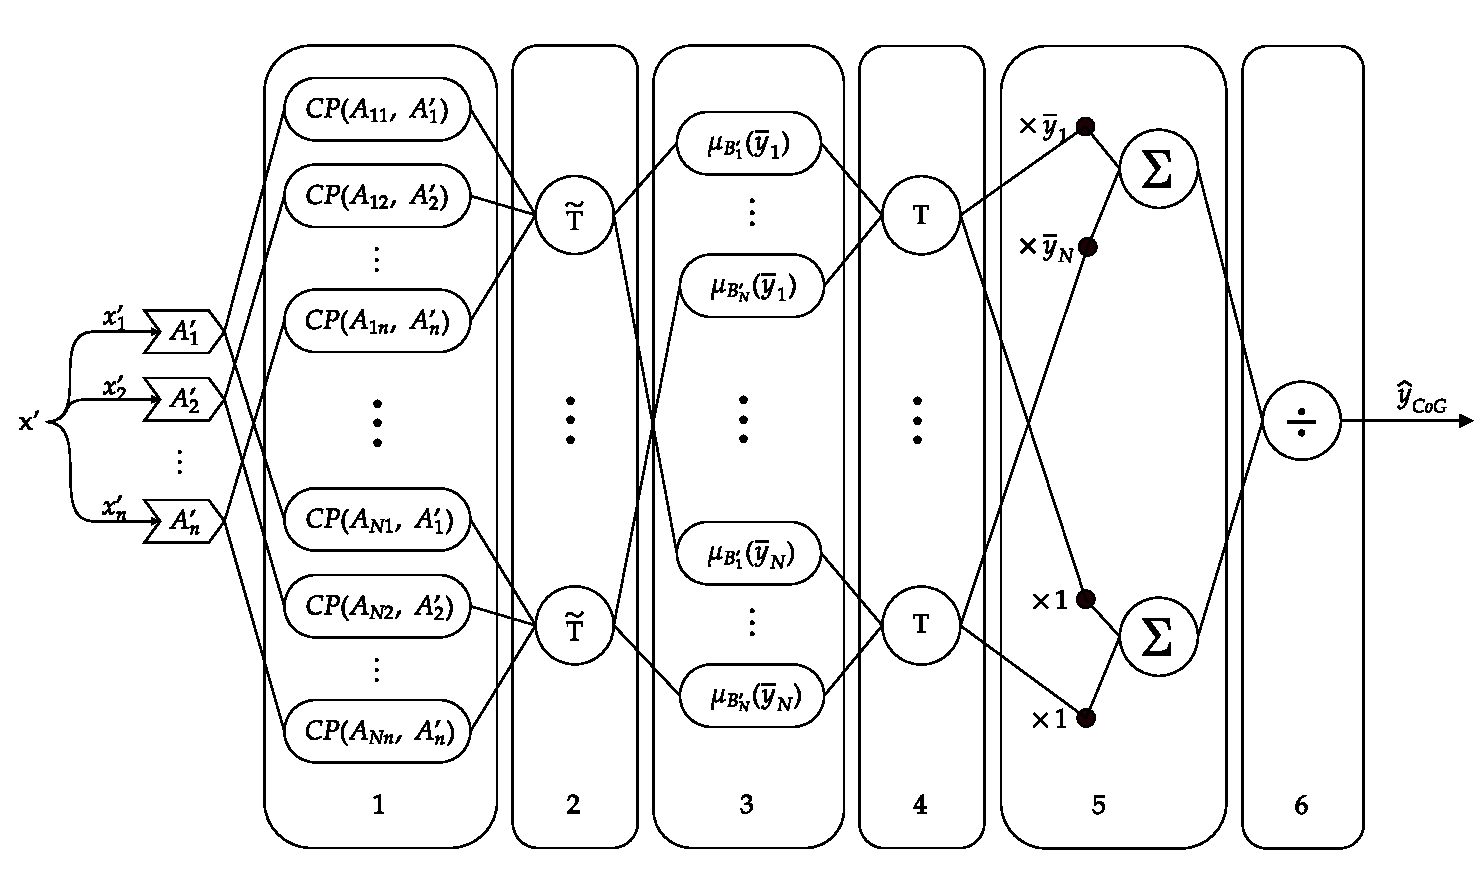
\includegraphics[scale=0.7]{neurofuzzysystem-defuzzification-cog}
	\caption{Схема нейро-нечеткой системы с использованием дефаззификации по методу центра тяжести}
	\label{fig:neurofuzzysystem-defuzzification-cog}
\end{figure}


\begin{figure}[ht]
	\centering
	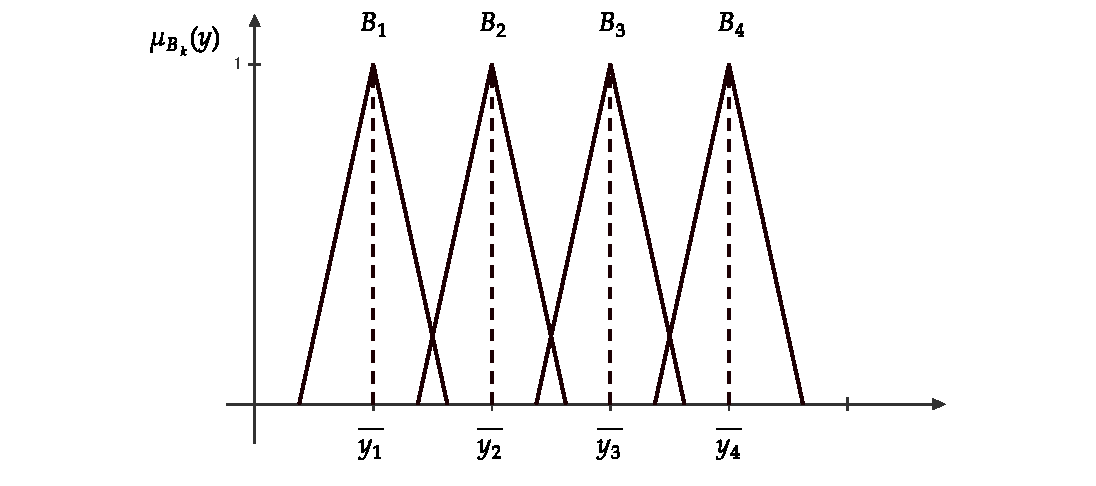
\includegraphics[]{out-mf-with-low-crossing}
	\caption{Пример нечетких множеств, удовлетворяющих условию $\mu_{B_k}(y_r) = 0$ для $y \ne r$}
	\label{fig:out_mf_with_low_crossing}
\end{figure}

Одна из возможностей упрощения процедуры вывода возникает, когда функции принадлежностей термов выходной лингвистической переменной достаточно удалены друг от друга и имеют низкую степень взаимного пересечения, то есть выполняется соотношение $\mu_{B_k}(y_r) \approx 0$ при $k \ne r$, что проиллюстрировано на рисунке \cref{fig:out_mf_with_low_crossing}.

Рассмотрим вычисление $\tau_{k\,r}$ для различных категорий импликаций:
\begin{itemize}
	\item для \textit{S}-импликации
	\begin{equation*}
		\tau_{k\,r}(v) = \begin{cases}
			1-v, & \quad \text{если } k \ne r \\
			1, & \quad \text{если } k = r
		\end{cases}
	\end{equation*}
	\begin{equation*}
		\hat{y}_{CoG} = \frac{\sum_{k=1}^{N} \overline{y}_k \Tnorm_{r=1}^N \left\{sup_{v\in [0, 1]} \left\{\tau_{A_r|A'}\overset{\mathrm{T}_2}{\star}(1-v)\right\}\right\}}{\sum_{k=1}^{N} \Tnorm_{r=1}^N \left\{sup_{v\in [0, 1]} \left\{\tau_{A_r|A'}\overset{\mathrm{T}_2}{\star}(1-v)\right\}\right\}},
	\end{equation*}
	\item для \textit{R}-импликации
	\begin{equation*}
	\tau_{k\,r}(v) = \begin{cases}
		\delta(v), & \text{если } k \ne r \\
		1, & \text{если } k = r
	\end{cases},
	\quad\text{где }
	\delta(v) = \begin{cases}
		1, & v = 0 \\
		0, & v > 0
	\end{cases}
	\end{equation*}
	\begin{equation*}
	\hat{y}_{CoG} = \frac{\sum_{k=1}^{N} \overline{y}_k \Tnorm_{r=1}^N \left\{\tau_{A_r|A'}(0)\right\}}{\sum_{k=1}^{N} \Tnorm_{r=1}^N \left\{\tau_{A_r|A'}(0)\right\}},
	\end{equation*}
	\item для \textit{S}-импликации
	\begin{equation*}
	\tau_{k\,r}(v) = \begin{cases}
		1-v, & \quad \text{если } k \ne r \\
		max(1-v, v), & \quad \text{если } k = r
	\end{cases}
	\end{equation*}
	\begin{equation*}
	\hat{y}_{CoG} = \frac{
		\sum_{k=1}^{N} \overline{y}_k \mathrm{T}_2 \left\{
			sup_{v\in [0, 1]} \left\{\tau_{A_k|A'}\overset{\mathrm{T}_2}{\star}max(1-v, v)\right\}
			\Tnorm_{\substack{r=1\\r\ne k}}^N \left\{
				sup_{v\in [0, 1]} \left\{\tau_{A_r|A'}\overset{\mathrm{T}_2}{\star}(1-v)\right\}
			\right\}
		\right\}
	}{
		\sum_{k=1}^{N} \mathrm{T}_2 \left\{
			sup_{v\in [0, 1]} \left\{\tau_{A_k|A'}\overset{\mathrm{T}_2}{\star}max(1-v, v)\right\}
			\Tnorm_{\substack{r=1\\r\ne k}}^N \left\{
				sup_{v\in [0, 1]} \left\{\tau_{A_r|A'}\overset{\mathrm{T}_2}{\star}(1-v)\right\}
			\right\}
		\right\}
	},
	\end{equation*}
\end{itemize}

\todo{Можно организовать вычисление всех значений $b_{k\,r}$ $\tau_{k\,r}$, но использовать разреженные матрицы в качестве структуры данных для хранения значений где $b_{k\,r} > 0$.}

\todo{Приведенные выклладки справедливы не только для функций принадлежностей отдельных термов, а и для набора кластеризованных в небольшие группы функций принадлжености со значительной степенью пересечения. При такой конфигурации выходного нечеткого пространства нет необходимости включать в процесс вывода правила, в которых функции принадлжености консеквента имеют низкий уровень пересечения с ф. п. правил, имеющих высокий уровень срабатывания для данного входа нечеткой системы.}

\subsection{Дефаззификация по методу центра области}

(center of area)

Данный метод можно сопоставить со схемой вычисления медианы случайной величины при заданном ее распределении. Формула вычисления дефаззифицированного значения $y^*_{CoA}$ имеет вид:

\begin{equation*}
\int_{\inf Y}^{\hat{y}_{CoA}} \mu_{B'}(y) dy = \int_{\hat{y}_{CoA}}^{\sup Y} \mu_{B'}(y) dy
\end{equation*}

\begin{align*}
\int_{\inf Y}^{\hat{y}_{CoA}} \Tnorm_{r=1}^N \left\{\sup_{v\in [0, 1]} \left\{\tau_{A_r|A'}\overset{\mathrm{T}_2}{\star} I\left(v, \mu_{B_r}(y)\right)\right\}\right\} dy =\\
= \int_{\hat{y}_{CoA}}^{\sup Y} \Tnorm_{r=1}^N \left\{\sup_{v\in [0, 1]} \left\{\tau_{A_r|A'}\overset{\mathrm{T}_2}{\star} I\left(v, \mu_{B_r}(y)\right)\right\}\right\} dy
\end{align*}

\subsection{Дефаззификация по методу среднего максимума}

\begin{equation*}
\hat{y}_{MeOM} = \frac{\sum_{x \in core(B')} x}{|core(B')|},
\end{equation*}
где $core(B') = \left\{y | y \in Y \textrm{ and } \mu_{B'}(y) = \sup_{y' \in Y} \mu_{B'}(y')\right\}$. 

Данный метод аналогичен по схеме вычисления моде случайной величины при заданном ее распределении. В случае унимодального вида функции принадлежности $\mu_{B'}(y)$ данный способ дефаззификации можно упростить до метода максимума функции принадлежности:
\[
\hat{y}_{MeOM} = \mathrm{arg\,max}_{y \in Y} \mu_{B'}(y).
\]

Тогда 


\section{Прогнозирование временных рядов на основе нечетких систем логическогго типа с использованием нечеткого значения истинности}

Для временного ряда $\mathbf{y_t} = (y_1, \dots, y_T)$ величина $y_t$ представляет измеренное значение наблюдаемой переменной в момент времени $t$. Ставится задача предсказания значений $\hat{y}_{t+h}$ для заданного горизонта предсказания $h$.

Модель временного ряда $f(\cdot)$ порядка $p$ использует последние $p$ значений до момента $t$ для оценки значения:
\[
	\hat{y}_{t+h} = f(y_{t-p}, \dots, y_t),
\]
где $p$ - размер лагового окна.

При моделировании временных последовательностей с использованием нейро-нечетких систем каждое значение $y_t\in Y$ фаззифицируется в нечеткое множество $A_t$. Эти нечеткие множества составляют множество термов лингвистической переменной $\tilde{A}$, определенной на базовом множестве $Y$. Такая система принимает $p$ входов, а правила в ее базе знаний устанавливают нечеткую последовательно-временную связь в рамках заданного окна $p+1$. Параметр $p$ называется порядком нечеткой системы прогнозирования временных рядов.

База правил в такой системе представляется набором из $N$ правил вида:
\begin{equation}
	\begin{aligned}
			R_k: \textrm{Если }&y_{t-p}\textrm{ есть }A_{k1}\textrm{ и }\dots\textrm{ и } y_{t}\textrm{ есть }A_{kp},&\\
			\textrm{ то }&y_{t+1}\textrm{ есть }A_{k\,p+1},&k\in\overline{1,N},
	\end{aligned}
\end{equation}
где каждое нечеткое отношение $\mathrm{T_1}\left\{A_{k1}, \dots, A_{kp}\right\} \rightarrow A_{k\,p+1}$, заданное в правиле $R_k$, выражает единицу \todo{логических} знаний о моделируемом протекающем во времени процессе.

Определив НЗИ $CP(\mathbf{A_{k}, \mathbf{A'}})$ для антецедента правила $R_k$ согласно (\ref{eqn:ftv-compute-12}) и (\ref{eqn:ftv-compute-8}), можно переписать правило $R_k$ в виде:
\begin{align*}
	R_k: \textrm{Если }&CP(\mathbf{A_{k}, \mathbf{A'}}),&\\
	\textrm{ то }&y_{t+1}\textrm{ есть }A_{k\,p+1},&k\in\overline{1,N}.
\end{align*}

\todo{Вычисленное значение истинности для каждого правила выражает соответствие среза измерений порождаемых некоторым величины некоторой единице знаний о динамике этого процесса.}

Если используется логический метод вывода на основе дефаззификации по центру тяжести, то согласно (\ref{}) нечеткий вывод выражается:
\begin{equation}
\hat{y}_{t+1} = \frac{\int_Y y_{t+1} \underset{k=\overline{1,N}}{\textrm{T}}\Biggl\{\sup_{v \in [0,1]}\biggl\{\tau_{\mathbf{A_k}|\mathbf{A'}}(v)\overset{T_2}{\star} I(v, \mu_{A_{k\,p+1}}(y_{t+1}))\biggr\}\Biggr\} dy_{t+1}}{\int_Y \underset{k=\overline{1,N}}{\textrm{T}}\Biggl\{\sup_{v \in [0,1]}\biggl\{\tau_{\mathbf{A_k}|\mathbf{A'}}(v)\overset{T_2}{\star} I(v, \mu_{A_{k\,p+1}}(y_{t+1}))\biggr\}\Biggr\} dy_{t+1}}
\end{equation}

Входы нечеткой системы по каждому измерению могут описываться одной и той же лингвистической переменной, заданной на базовом множестве области значений временного ряда и имеющей одинаковую порождающую процедуру для терм-множеств.

\todo{Обучение нечетких систем прогнозирования временных рядов .} Ранние подходы следовали более типовому набору шагов для построения нечетких систем \cite{Chellai2022}: пространство значений временного ряда разбивалось на пересекающиеся участки для формирования термов единственной лингвистической переменной $\tilde{A}$, а база правил формировалась по принципу наибольшей степени принадлежности для каждого экземпляра входных данных, например, с помощью популярного из-за своей простоты метода \cite{Wang1992}. В широко цитируемом подходе Чена \cite{Chen1996} разбиение производилось на равные отрезки. В более поздних методах формирование сразу базы правил с соответствующими терм-множествами из данных, то есть более точное выделение шаблонных отрезков из временных рядов, стало более распространенным подходом, из-за ограничений в увеличении точности нечеткой системы при разбиения базового множества лингвистической переменной $\tilde{A}$ со сложной функцией плотности распределения значений. Таким образом одни и те же методы можно применять для разбиения пространства значений временных рядов (одно измерение) или для разделения пространства окон временных рядов (когда последовательность значений в окне временного ряда интерпретируется как точка в $n$-мерном пространстве). В последнем случае посредством разбиения пространства окон временного ряда может осуществляться формирование базы правил.

Распространенной группой таких методов являются подходы на основе различных алгоритмов кластеризации \cite{Lucas2021}:  \textit{k}-средних, алгоритмы учитывающие плотность распределения точек, агломеративная кластеризация. Эволюционные подходы, например, Particle Swarm Optimization (PSO).

Стоит также отметить гибридные подходы построения и обучения нечетких систем моделирования временных рядов в комбинации с другими моделями машинного обучения, такими как, Support Vector Machine (SVM), Long-Sort Term Memory (LSTM), Transformer, и статистические методели, например, Auto Regressive Integrated Moving Average (ARIMA).

Отдельно прорабатываются подходы потокового обучения нечетких систем\cite{Lima2010, Alves2021} для непрерывного поступающего потока данных.

Для реализации сильных сторон от использования нечеткого моделирования нужно отразить информацию о прогнозируемой величине при выборе метода ее фаззификации. Существующие подходы фаззификации значений временных рядов комбинируют различные формы функций принадлжености, способы оценку истинного значения в термах и формализации неопределенности. В \cite{Pekaslan2020} описан подход к фаззификации измеренных значений временного ряда в нечеткие множества с гауссовыми  функциями принадлежности. Измеренные значения полагаются истинными и задают центры гауссовых функций принадлежности, а среднеквадратичное отклонение оценивается как среднеквадратичная разность между соседними значениями в некотором окне вокруг данной точки во временной последовательности. \todo{Написать формулу} В \cite{Pourabdollah2017} для фаззифицированных таким образом значений в нечеткие множества выполняется переоценка истинных значений посредством преобразования взвешенным скользящим средним центров гауссовой ф. п. нечетких множеств. \todo{Написать формулу} Стоит уточнить, что в этих двух работах рассматривается нечеткий вывод с использованием non-singleton фаззификации.

Для выбора используемой импликации и метода дефаззификации изучен анализ точности в задаче регрессии приведенный в работах \cite{Kiszka1985} и \cite{} соответственно.


\section{Выводы}

В главе приведена постановка задачи нечеткого логического вывода в канонической форме Заде. Затем описана альтернативная схема нечеткого логического вывода с использованием нечеткого значения истинности, в которой база правил приобретает новую структуру правил вида: <<Если \textit{истинно}, то $B_k$>>. Также формально описана схема вычисления свертки НЗИ на основе НЗИ по отдельным входам с помощью расширенной $t$-нормы --- $\tilde{\mathrm{T}}$.

\todo{Проведен анализ\dots}

В главе приведены итоговые формулы нечеткого вывода на основе нечеткого значения истинности для различных методов дефаззификации. Также выведены упрощенные формулы вычисления дефаззифицированного значения для различных специальных категорий импликаций.

Дано формальное описание применения разработанной модели нечеткого логического вывода в задаче прогнозирования временных рядов. Приведены существующие подходы фаззификации значений временных рядов и методы автоматического подбора параметров термов лингвистической переменной и формирования базы правил на основе наборов обучающих данных.

\FloatBarrier
